\chapter{Flots de liens: extension temporelle des graphes}
\minitoc
\label{chap:def_flot}

\section{Définition}
\label{sec:definition}

Nous avons décrit le formalisme de flot de liens dans le chapitre précédent.
Nous nous attachons maintenant à définir plus formellement les flots de liens et quelques notions utilisées dans le reste de cette thèse.
Un flot de liens est défini par un triplet $L=(T,V,E)$ où $T=[\alpha, \omega]$ est un intervalle de temps, $V$ un ensemble de $n$ n\oe{}uds et $E\subseteq T\times T \times V \times V$ un ensemble de $m$ liens.
Les liens de $E$ sont des quadruplets $(b,e,u,v)$, signifiant que le lien $(u, v)$ existe sur l'intervalle $[b,e] \subseteq [\alpha,\omega]$.
Nous notons le nombre de liens dans le flot par $|L|=|E|=m$ et sa durée par $\bar{L}=\omega-\alpha$.
De manière analogue, la durée d'un lien $l=(b,e,u,v) \in E$ est notée   $\bar{l}=e-b$.
On note $\beta(E)= min_{(b,e,u,v) \in E} (b)$ et $\psi(E)= max_{(b,e,u,v) \in E} (e)$ l'apparition du premier lien et la disparition du dernier lien dans le flot de liens.

Nous considérons les flots de liens non orientés et sans boucles, \emph{i.e.}$(b,e,u,v)=(b,e,v,u)$ et $u \neq v$.
Enfin de manière analogue aux graphes et aux multigraphes, nous définissons les flots de liens simples.
Un flot de liens est simple si pour tout $l_1=(b,e,u,v) \in E$ et $l_2=(b',e',u, v) \in E$, $[b,e]\cap [b', e'] = \emptyset$ si $l_1 \neq l_2$.
Dans les graphes, il est possible de transformer un multigraphe en graphe simple.
Nous définissons également cette opération que nous nommons simplification: $\sigma(L)$.
Afin de définir la simplification, nous nous aidons de la fonction de présence $\zeta_{L}(u,v,t)$ d'un flot de liens qui est égale à $1$ si au moins un lien existe dans $L$ entre $u$ et $v$ à l'instant $t$ et $0$ sinon.
$L'=(T,V,E')= \sigma(L)$ est la simplification de $L=(T,V,E)$ si et seulement si $L'$ est simple et si $\forall u,v \in V,\ \forall t\in T, \zeta_{L}(u,v,t)= \zeta_{L'}(u,v,t)$.

Il est parfois nécessaire d'augmenter la durée de chaque lien.
C'est notamment utile lorsque les liens sont de la forme $(t,t,u,v)$, ce qui est le cas lorsqu'on étudie des envois de courriels par exemple.
Nous notons $\xi(L,\Delta)$ l'augmentation de la durée de chaque lien de $\Delta$.
Il y a plusieurs moyens d'augmenter de $\Delta$ un intervalle $[b,e]$.
Nous considérons l'ajout symétrique c'est à dire qu'un intervalle $[b,e]$ est transformé en l'intervalle $[b-\Delta/2,e+\Delta/2]$.

Enfin, il est parfois intéressant d'agréger l'information temporelle pour créer un graphe statique.
Un graphe $G=(V,E')=G(L)$ est le graphe agrégé de $L$ si et seulement si $\forall (u,v) \in E',\ \exists b,e \in T$ tel que $(b,e,u,v) \in E$ et réciproquement.


%Une fois défini les flots de liens, nous pouvons commencer à définir différentes opérations pour les analyser.


\section{Sous-flots}
Dans les graphes, il existe la notion de sous graphes, voir la section~\ref{sec:def_graphe}, que nous étendons également aux flots de liens.
Un flot de liens $L'=(T',V',E')$ est un sous-flot de $L$, ce que l'on note $L' \subseteq L$, si et seulement si $T'\subseteq T$, $V'\subseteq V$ et  $\forall u,v \in V,\ \forall t\in T, \zeta_{L'}(u,v,t) \leq \zeta_{L}(u,v,t)$.
Cette notion est en particulier utile pour définir des sous-flots induits par différents ensembles d'éléments.
Nous illustrons ces notions dans les figures~\ref{fig:exemple_sous_flot1} et \ref{fig:exemple_sous_flot2} avec le flot initial dans la figure~\ref{fig:exemple_sous_flot_init}.
 
Nous définissons $L(E')$ , le sous-flot de $L$ induit par un ensemble de liens $E' \subset E$: $L(E')=([\beta(E'),\psi(E')],V(E'),E')$ où $V(E')=\{u, \exists (b,e,u,v) \in E\}$ est l'ensemble des n\oe{}uds induits par $E'$.

 
Nous définissons $L(S)$ , le sous-flot de $L$ induit par un ensemble de paires de n\oe{}uds $S \in V2$: $L(S)=([\beta(E'),\psi(E')],V',E')$ avec $E'= \{(b,e,u,v) \in E, (u,v) \in S\}$ et $V'=\{u, \exists (u,v) \in S\}$.
Par convention, on note $L(v)= L(\{v\}\times V)$, le sous-flot induit par un n\oe{}ud.
Un exemple de sous-flot induit par un n\oe{}ud est dans la figure~\ref{fig:exemple_sous_flot1}.


Enfin, nous définissons $L_{t..t'}=([t, t'], V,E')$, le sous-flot de $L$ induit par l'intervalle de temps $[t,t'] \subset [\alpha, \omega]$ où $E'= \{(b',e',u,v),\ \exists (b,e,u,v) \in E,\ b'= max(b,t),\ e'=min(e,t'),\ [b,e]\cap [t,t']\neq \emptyset\}$.
Il est également possible de définir $L_{t..t'}$ via la fonction de présence: $\forall u,v \in V,\ \forall x \in [t,t']\  \zeta_{L_{t..t'}}(u,v,x) = \zeta_{L}(u,v,x)$.
Tous les liens qui sont présents durant au moins un instant de l'intervalle $[t, t']$ sont dans le sous-flot.
Un exemple de sous-flot induit par un intervalle de temps est présenté dans la figure~\ref{fig:exemple_sous_flot2}.
Il est intéressant de noter que le sous-flot $L_{t..t}$, que l'on note $L_t$, est équivalent au graphe statique à l'instant $t$,  que nous notons $G(L_t)$.
Ce graphe statique à un instant correspond au formalisme de graphe temporel présenté précédemment.


\begin{figure}[]
\centering
	\begin{subfigure}{0.25\linewidth}
		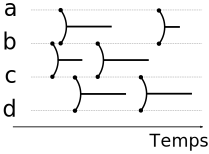
\includegraphics[width=\linewidth]{img/Intro/sous_flots.eps}\hfill
		\caption{Flot de liens initial $L$}
		\label{fig:exemple_sous_flot_init}	
	\end{subfigure}\hspace{0.1\linewidth}
	\begin{subfigure}{0.25\linewidth}
		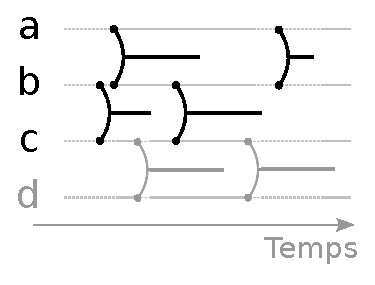
\includegraphics[width=\linewidth]{img/Intro/sous_flots1.eps}\hfill
		\caption{Sous-flot induit par des n\oe{}uds: $L(b)$}	
		\label{fig:exemple_sous_flot1}	
	\end{subfigure}\hspace{0.1\linewidth}
	\begin{subfigure}{0.25\linewidth}
		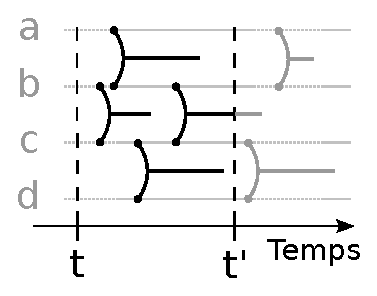
\includegraphics[width=\linewidth]{img/Intro/sous_flots2.eps}\hfill
		\caption{Sous-flot induit par le temps:  $L_{t..t'}$}
		\label{fig:exemple_sous_flot2}	
	\end{subfigure}
	\caption{Exemple de différents sous-flots, (B) et (C), du flot initial en (A). Les liens en noirs sont les liens sélectionnés dans le sous-flot. }
\label{fig:exemple_sous_flot}
\end{figure}
Enfin, il est aussi possible de combiner ces notions.
Par exemple avec $V' \subset V$, $L_{t..t'}(V'\,^2)$ est le sous-flot correspondant aux liens entre les n\oe{}uds de $V'$ sur l'intervalle $[t, t']$.

\bigskip

Un sous-flot induit par un ensemble de paires de n\oe{}uds peut être construit de manière quasiment linéaire en nombre de liens dans le sous-flot.
Pour un ensemble de paires de n\oe{}uds $S= V_1 \times V_2$, il suffit d'itérer sur l'ensemble des liens qui sont reliés aux n\oe{}uds de $V_1$ et de vérifier que l'autre n\oe{}ud du lien appartient à $V_2$. ce qui se fait en $O(\log(|V_2|))$ pour chaque lien.
Le parcours des liens reliés à $V_1$ peut être fait en $O(|L(V_1 \times V)|)$ si chaque n\oe{}ud a la connaissance des liens auxquels il est relié.
Si tel est le cas alors il est possible de construire le sous-flot en $O(|L(V_1\times V)|\log(|V_2|))$.
Il faut tout de fois distinguer le cas où $S= V_1 \times V$ car il n'est alors pas nécessaire de faire la vérification et la complexité est alors $O(|L(V_1\times V)|)$.

Pour l'intervalle de temps, la situation est plus compliquée car il n'est pas facile de connaître l'ensemble des liens existant à un instant donné.
Il est possible de les trier par ordre d'apparition ou de disparition mais il n'y a pas d'ordre total sur la présence des liens.
Pour qu'un lien, $l= (b,e,u,v)$ appartienne au sous-flot temporel sur $[t,t']$, il doit remplir les deux conditions suivantes:
\begin{itemize}
\item \textbf{$b \leq t'$} le lien commence avant la fin de l'intervalle $[t,t']$.
\item \textbf{$e \geq t$} le lien finit après le début de l'intervalle $[t,t']$.
\end{itemize}


Il n'est donc pas nécessaire de considérer les liens ayant un temps de fin inférieur à $t$.
De manière analogue, il n'est pas nécessaire de considérer les liens ayant un temps de début supérieur $t'$.
Cependant ces deux conditions ne peuvent pas être combinées pour restreindre le nombre liens considérés.
Une manière de construire le sous-flot temporel est d'itérer sur tous les liens dans l'ordre temporel d'apparition et d'arrêter le parcours dès qu'un lien a un temps de début supérieur à $t'$.
Il faut cependant tester l'appartenance de chaque lien parcouru.
Il n'est pas possible de restreindre d'avantage le parcours car l'ensemble des liens débutant entre $\alpha$ et $t$ peuvent être dans le sous-flot en respectant la dernière condition.
De manière analogue, il est possible d'itérer sur les liens dans l'ordre inverse de disparition des liens et de s'arrêter dès qu'un lien a un temps de fin inférieur à $t$.


Dans le pire des cas, ces méthodes sont donc linéaires sur le nombre total de liens dans le flot et non dans le sous-flot comme précédemment.
Il n'y a alors que deux optimisations possibles.
Il est possible de choisir le sens du parcours si les deux ordres sont disponibles.
Si la plus longue durée de liens, $\bar{l}_{max}$, est connue, alors il est possible de commencer la recherche à partir du premier lien respectant $b+\bar{l}_{max} \geq t$.



\section{Degré et densité}
\label{sec:def_densite}
Nous avons défini des outils pour manipuler et extraire des sous-flots d'un flot de liens.
Nous nous intéressons maintenant à étendre quelques notions existantes dans les graphes, en particulier le degré et la densité.


Il est assez trivial de définir le degré temporel d'un n\oe{}ud $u$ de la manière suivante:
\begin{equation}
d(t,u)= |L_t(u)|= \sum_{v \in V} \zeta_{L}(u,v,t).
\end{equation}
Le degré temporel n'est alors pas une valeur comme dans les graphes mais une fonction qui dépend du temps.
Comme les liens apparaissent et disparaissent de manière instantanée, la fonction de degré est une fonction constante par morceaux.
Un exemple de degré temporel est présenté dans la figure~\ref{fig:exemple_degre}.

\begin{figure}
\centering
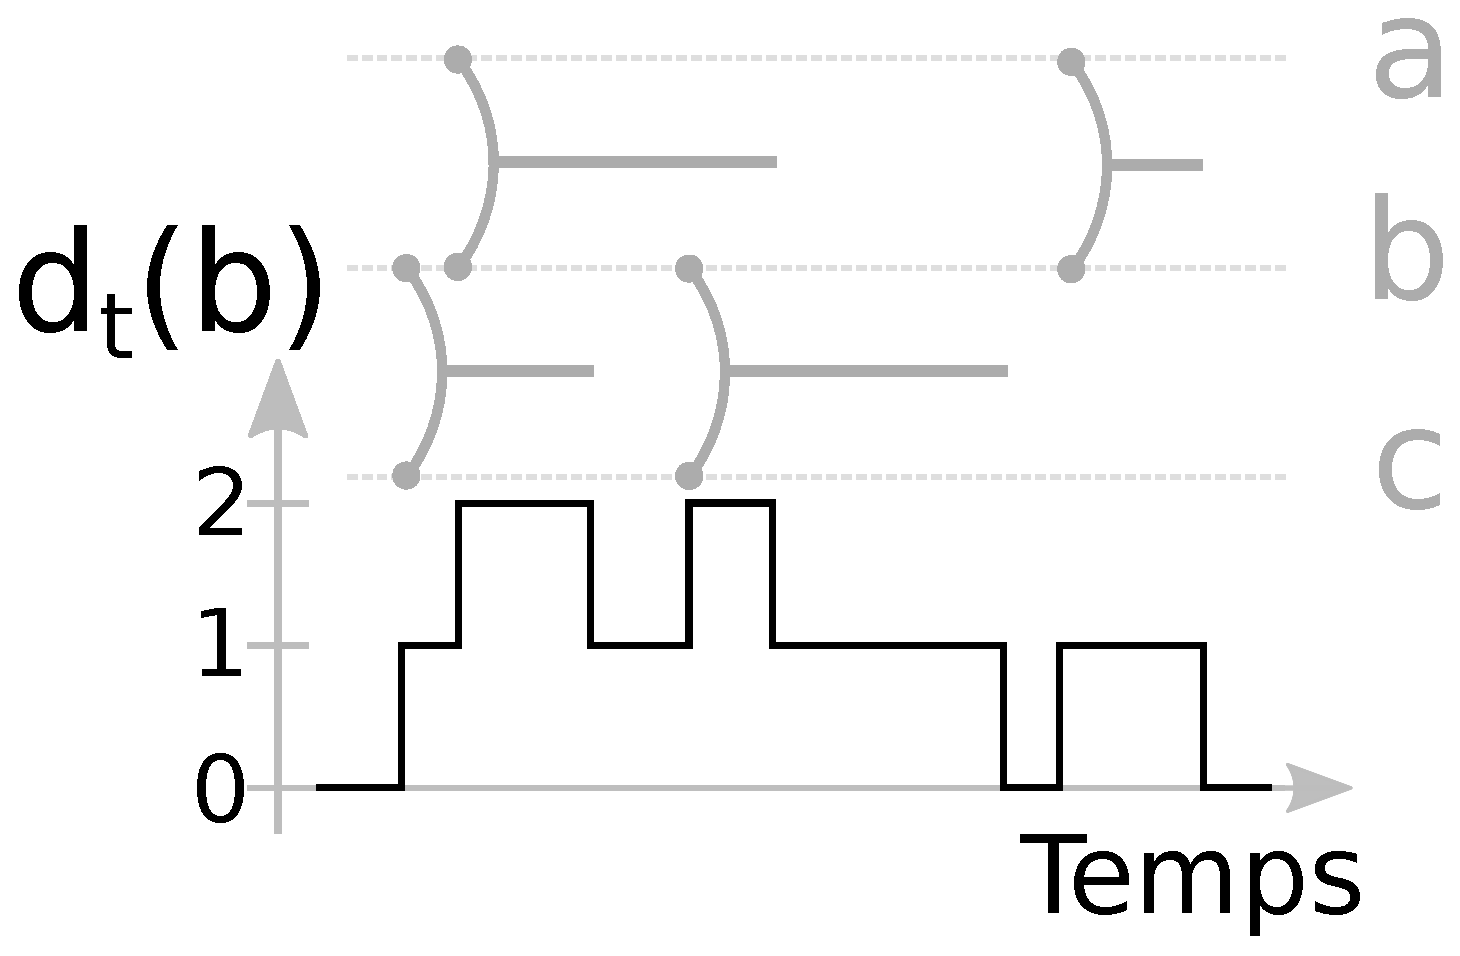
\includegraphics[width=0.35\linewidth]{img/Intro/degre2.eps}
\caption{Degré temporel du n\oe{}ud $b$ dans le flot de liens dans la figure~\ref{fig:exemple_sous_flot_init} qui est également rappelé en grisé dans cette figure.
}
\label{fig:exemple_degre}
\end{figure}

De manière analogue aux graphes, il est également possible de définir le degré temporel d'un ensemble de n\oe{}uds, $d_t(V')$ , ou d'un ensemble de liens, $d_t(E')$:

\begin{equation}
d(t, V') = \sum_{v \in V'} d(t,v) = 2 |L_{t}(V'\times V')|+ |L_{t}(V'\times V \setminus V')|\,,
\end{equation}

\begin{equation}
d(t, E')=2|L_{t}(E')| \,.
\end{equation}

Avec ces définitions, il est aussi possible définir les notions de degré temporel interne, $d_{in}(t,V') = 2 |L_{t}(V'\times V')|$, et externe $d_{out}(t,V')=|L_{t}(V'\times V \setminus V')|$.
Les degrés temporels d'un n\oe{}ud, d'un ensemble de n\oe{}uds ou de liens peuvent se calculer rapidement.
Il faut pour ce faire considérer les liens appartenant au sous-flot induit respectivement par un n\oe{}ud, ensemble de liens ou un ensemble de paires de n\oe{}uds.
Il faut d'abord transformer les liens $(b,e,u,v)$ du sous-flot en une suite de modifications de la forme $(b,+1)$ et $(e,-1)$ ce qui a une complexité en $O(m)$.
Une fois cette liste créée, il suffit d'ordonner ces modifications dans l'ordre temporel, ce qui peut être fait en temps $O(2m\log(2m))$, puis d'itérer sur l'ensemble des modification en sommant au fur et à mesure les apparitions et disparitions de lien, ce qui peut être fait en temps $O(2m)$.
Ainsi, le degré temporel à un instant $t$ est égal à la valeur de la somme des modification à cet instant.
\bigskip

Les degrés sont des fonctions du temps mais il est souvent intéressant de regarder la somme pondérée du degré, que l'on note $D_{t..t'}(u)$, et le degré moyen, que l'on note $d_{t..t'}(u)$, sur un intervalle donné:
\begin{equation}
D_{t..t'}(u)= \int_{t}^{t'}d(t,u) dt  = \sum_{l \in L_{t..t'}(u)}\bar{l} \qquad
d_{t..t'}(u)= \dfrac{D_{t..t'}(u)}{t'-t}\, .
\label{eq:deg_moyen}
\end{equation}

Lorsque cela n'est pas ambigu, nous notons $d_{\alpha..\omega}(u) = d(u)$.
Il est intéressant de noter dans cette formulation que si tous les liens durent tout au long du flot de liens alors le degré dans le graphe agrégé et le degré moyen dans le flot de liens sont égaux, c'est-à-dire  $d_{\alpha..\omega}(u) = d_{G(L)}(u), \forall u \in V$.

\`A partir du degré, il est possible de définir beaucoup de notions différentes et notamment la densité.
Pour rappel, la densité dans un graphe est définie par $\delta(G)=2m/(n(n-1))=d(V)/n(n-1)$ et est égale à la probabilité qu'il existe un lien entre 2 n\oe{}uds pris au hasard.
Si l'on transpose l'idée au formalisme de flot de liens, la densité dans un flot de liens est la probabilité qu'il existe un lien entre 2 n\oe{}uds à un instant donné aléatoire.
Cela se traduit par la formule suivante:
\begin{equation}
\delta(L)= \dfrac{2 \sum_{l \in E}\bar{l}}{n(n-1) (\omega-\alpha)}.
\end{equation}

Cette formulation est équivalente à la densité moyenne des graphes $G(L_t)$:

\begin{equation*}
\dfrac{1}{\omega-\alpha} \int_{\alpha}^{\omega} \delta(G(L_t)) dt=
\dfrac{1}{\omega-\alpha} \int_{\alpha}^{\omega} \dfrac{d(t,V)}{n(n-1)}dt=
 \dfrac{1}{\omega-\alpha} \int_{\alpha}^{\omega} \dfrac{\sum_{u \in V} d(t,u)}{n(n-1)}dt
 \end{equation*}

 \begin{equation*}
= \dfrac{\sum_{u \in V} \int_{\alpha}^{\omega}d(t,u)dt}{n(n-1)(\omega-\alpha)} =
\dfrac{\sum_{u \in V} \sum_{l \in L_(u)} \bar{l}}{n(n-1)(\omega-\alpha)} =
\dfrac{2\sum_{l \in E}\bar{l}}{n(n-1) (\omega-\alpha)} .
\end{equation*}

Pour arriver à ce résultat, nous utilisons la relation entre degré temporel moyen et somme des durées de l'équation~\ref{eq:deg_moyen}.

La notion de densité que nous avons définie est donc cohérente avec notre notion de degré et traduit le même concept que dans les graphes.
Ainsi, la densité dans les flots de liens est aussi comprise entre à $0$ et $1$.
Enfin, cette formulation de densité est une généralisation de la densité proposée par Viard~\emph{et al.}~\cite{Viard2014a} qui ne considérait que les liens sans durée.
Les auteurs considèrent l'ajout de temps arbitraire sur chaque lien.
Leur formulation est équivalente à la densité suivante: $\delta( \sigma(\xi(L,\Delta)))$ si l'augmentation de la durée ne se fait pas de manière symétrique.
Un lien est $(t,t,u,v)$ est transformé en un lien $(t-\Delta,t,u,v)$.

Le calcul de la densité d'un flot est linéaire en le nombre de liens car il est dépendant du calcul de $d_{\alpha..\omega}(V)$  qui est fait de manière linéaire.


\begin{table}
	\centering
	\begin{tabular}{|c|c|}
	\hline Symbole & description \\
	\hline $L$ & Flot de liens \\ 
	$T$ & intervalle de temps  \\
	$V$ & ensemble de n\oe{}uds\\
	$E$ & ensemble de liens: $(b,e,u,v)$ \\
	$|L|,|E|$ & nombre de liens dans le flot \\
	$\beta(E)$ & temps d'apparition du premier lien\\
	$\psi(E)$ & temps de disparition du dernier lien\\
	$\xi(L,\Delta)$ & augmentation de la durée de chaque lien de $\Delta$\\
	$\sigma(L)$ & Simplification du flot de liens $L$\\
	$G(L)$ & graphe agrégé de $L$\\
	$L(V_1\times V_2)$ & sous-flot induit par l'ensemble de paires de n\oe{}uds $V_1\times V_2$ \\
	$L_{t..t'}$ & sous-flot induit par l'intervalle $[t,t']$ \\
	$L_{t}$ & sous-flot induit par un instant $t$\\
	$d_t(v)$ & degré de $v$ à l'instant $t$\\
	$d_t(V)$ & somme des degrés des n\oe{}uds dans $V$ à l'instant $t$\\
	$d_{in}(t,V')$ & somme des degrés internes des n\oe{}uds dans $V'$ à l'instant $t$\\
	$d_{t..t'}(v)$ & degré moyen de $v$ sur $[t,t']$\\
	$D_{t..t'}(u)$ & somme pondérée du degré de $v$ sur $[t,t']$\\
	$d(v)$ & degré moyen $v$ sur $T$\\
	$\delta(L)$ & densité du flot\\
%	$\delta_{\Delta}(L)$ & densité du flot où chaque lien dure $\Delta$\\
	\hline
	\end{tabular} 
		\caption{Liste des notations pour les flots de liens}
\end{table}

\bigskip
D'autres notions ont par ailleurs été définies dans les flots de liens  dans la thèse de Tiphaine Viard~\cite{viard2016flots}.

\section{Manipulation concrète des flots de liens}

Nous avons défini formellement quelques notions pour les flots de liens.
Afin de manipuler ces notions simplement, nous avons mis en place une librairie capable de les calculer.
Le but est de fournir une implémentation générale qui soit simple d'accès.
Ainsi, il sera possible à n'importe qui de calculer ces notions.
La démarche, bien que beaucoup plus modeste, est similaire à ce qui est fait pour les graphes avec \emph{networkx}\,\footnote{\url{https://networkx.github.io/}}.

L'implémentation est en \emph{C++} pour la rapidité avec un export en \emph{python} pour faciliter l'utilisation.
Le code de cette implémentation est en ligne\,\footnote{\url{https://bitbucket.org/nGaumont/liblinkstream/}} et la documentation également\,\footnote{\url{https://linkstream.ngaumont.fr/}}.
Il est, par exemple, possible avec la librairie de lire un flot de liens et de calculer la densité moyenne d'un sous-ensemble de n\oe{}uds sur un intervalle arbitraire.
Comme le but de cette librairie est d'être généraliste, l'implémentation n'est pas optimisée pour un calcul spécifique.
Ainsi, il est aisé d'étendre la librairie afin de permettre le calcul de nouvelles notions.
 

Un intérêt de cette implémentation est de permettre, en python, la génération de visualisation\,\footnote{Pour  l'instant, uniquement un export en svg est possible.}, voir le dessin dans la figure~\ref{fig:exemple_Flot_de_liens_lib}.
Parmi les possibilités offertes par la visualisation, il est possible de n'afficher qu'une partie des n\oe{}uds ou de ne garder qu'un sous intervalle de temps.
De plus, il est possible de choisir la couleur des liens de manière manuelle ou en fonction d'une partition de liens.

\begin{figure}
\centering
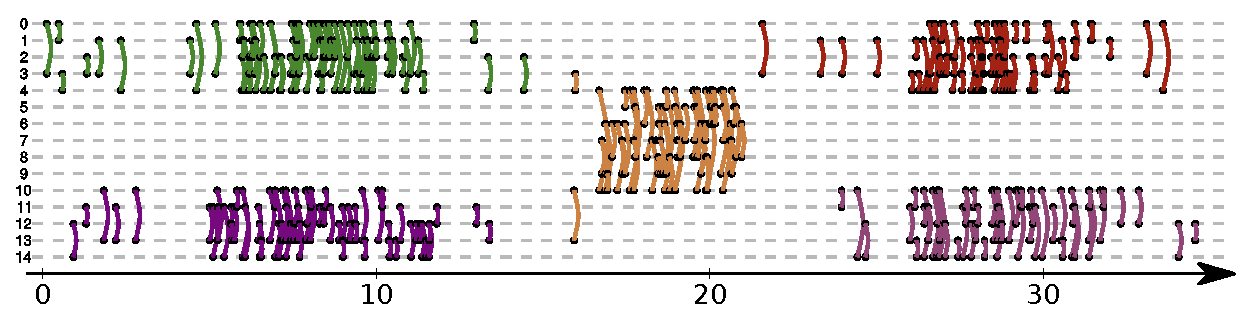
\includegraphics[width=\linewidth]{img/Intro/Dessin_Flot.eps}
\caption{Exemple d'une visualisation d'un flot de liens sans durées entre $15$ n\oe{}ds au cours du temps qui a été généré par notre librairie.
La couleur des liens a été fixée par l'utilisateur de la librairie.
}
\label{fig:exemple_Flot_de_liens_lib}
\end{figure}

La lisibilité de ce genre de visualisation est très dépendante de l'ordre attribué aux n\oe{}uds sur l'axes des ordonnées.
C'est pourquoi avec notre outil, il est également possible de fixer un ordre arbitraire.
Comme il peut être fastidieux d'écrire un ordre, nous avons implémenté un algorithme rudimentaire pour améliorer l'ordonnancement des n\oe{}uds dans la visualisation.
Afin de pouvoir améliorer une visualisation, il est nécessaire de pouvoir quantifier la complexité de la visualisation actuelle.
Empiriquement, on se rend vite compte que ce sont les longs traits verticaux qui rendent la visualisation complexe.
Il faut donc les limiter.

C'est pourquoi nous décidons d'évaluer un ordonnancement par la somme des longueurs des traits représentant les liens.
Avec la fonction d'ordre $Ordre: V \longmapsto \mathbb{N}$, trouver le meilleur ordonnancement se résume à résoudre:

\begin{equation}
 Ordre* = \argmin_{Ordre}  \sum_{(b,e,u,v) \in E} |Ordre(u)- Ordre(v)|
\end{equation}

Malheureusement, trouver l'optimum ne semble pas trivial et il n'est pas envisageable de tester l'ensemble des ordres.
C'est pourquoi nous utilisons un algorithme probabiliste qui teste des permutations aléatoires.
Une permutation est appliquée si elle améliore l'évaluation de la visualisation.
Il s'agit bien sûr d'une première approche qu'il est possible d'améliorer.

Une piste possible est la construction d'un ordre potentiellement proche de l'optimum.
Par exemple, il serait intéressant de trier chaque paire de n\oe{}uds $(u,v)$ en fonction du nombre de liens existants entre $u$ et $v$ puis de construire itérativement un ordre des n\oe{}uds en fonction de l'ordre des paires de n\oe{}uds.
